\section*{Harp Mini\-Batch Kmeans}

\TODO{Hyungro: check hyperlinks}

The goal for this exercise is to implement Harp Mini-batch Kmeans
from scratch (See~\hyperlink{link_exercise8}{Useful Links}). 

\subsection*{Deliverables}
Zip your source code and report as username\_mbkmeans.zip. Please submit this
file to the Canvas Assignments page.

\subsection*{Evaluation}

The point total for this exercise is 6, where the distribution is as
follows:

\begin{itemize}
\item Completeness of your code (5 points)
\item In the report, describe your implementation and the output. (1 points)
\end{itemize}

You can get up to 4 bonus points based on your extra efforts.

\section*{Bonus credits}

Some options you may consider to get extra credits: 

\begin{itemize}
\item Perform experiments on various (small, medium, large, etc)
  datasets
\item Test your algorithm on at least 2 nodes on FutureSystem.
\item Implement mini-batch kmeans using other tools/platforms (Spark,
  Flink, etc) and compare the performance between different
  tools/platforms (See~\hyperlink{link_exercise8}{Useful Links}).
\end{itemize}

You are encouraged to explore other options to get extra
credits. Remember to present all of your extra work in the report.
 
\subsection*{Dataset}

You can implement a script to generate data randomly as your input
datasets.  You are also free to use public datasets such as RCV1-v2
(See~\hyperlink{link_exercise8}{Useful Links}).
  
\subsection*{Mini-batch Kmeans}

You can refer to the paper for sequential mini-batch kmeans
algorithm. You will need to design how to parallelize the algorithm so
that it can run with large scale datasets on distributed computing
environment.

\begin{figure}[htb]
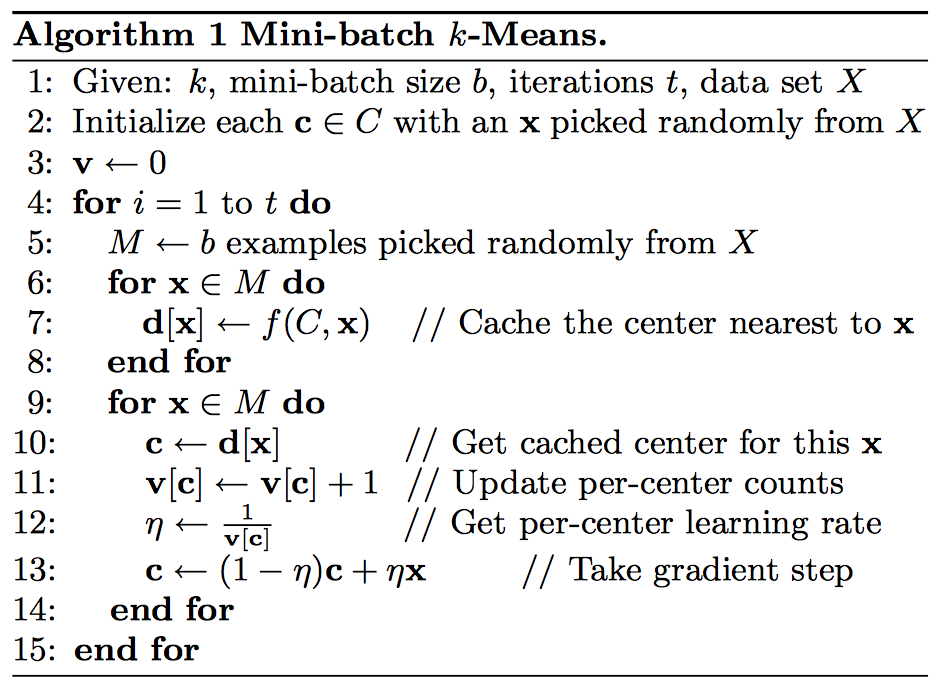
\includegraphics[width=8cm]{section/icloud/assignment/problems/exercise8/mbkmeans}
\centering
\caption{Mini-batch Kmeans.}
\end{figure}  

\subsection*{Useful Links}

\begin{itemize}
  \item \href{http://jmlr.csail.mit.edu/papers/volume5/lewis04a/lewis04a.pdf}{RCV1: A New Benchmark Collection for Text Categorization Research} \hypertarget{link_exercise8}
  \item \href{https://dsc-spidal.github.io/harp}{Harp}
  \item \href{http://spark.apache.org}{Spark}
  \item \href{https://flink.apache.org}{Flink}
  \item \href{https://dl.acm.org/citation.cfm?id=1772862}{Web-scale k-means clustering - D. Sculley}
\end{itemize}
